\section{Planiranje}

\textbf{plan} zaporedje akcij, ki pripelje od zacetnega do koncnega stanja

\subsection{Planiranje s sredstvi in cilji (STRIPS)}
Agentu opisemo svet in postavimo fizikalne omejitve.\\
Ne zagotovalja optimalne resitve, obravnavamo le en cilj naenkrat (ko ga dosezemo, se lahko ostali izgubijo) = Sussmanova anomalija\\
\green{Akcija} move(X, From, To)
\begin{itemize}[noitemsep,topsep=0pt,leftmargin=*]
    \item pogoj: \blue{cond}=[clr(X), on(X,F), clr(T)] $\rightarrow$ pogoji za izvajanje akcije,
    \item poz. ucinki: \blue{adds}=[on(X, T), clr(F)] $\rightarrow$ nova stanja,
    \item neg. ucinki: \blue{dels}=[on(X, F), clr(T)] $\rightarrow$ izbrisana stanja,
    \item omejitve: \blue{constr}=[F $\neq$ T, X$\neq$ F, X$\neq$ T, block(X)] $\rightarrow$ omejitve akcij (fizikalne omejitve),
\end{itemize}
\cyan{Algoritem}:
\begin{enumerate}[noitemsep,topsep=0pt,leftmargin=*]
    \item Izberi se neresen cilj iz mnozice CILJEV
    \item Izberi akcijo, ki izbrani cilj doda v stanje
    \item Omogoci izbrano akcijo (izpolni pogoje)
    \item Izvedi akcijo (ki izopolni najvec pogojev)
    \item Ce obstajajo nereseni cilji $\Rightarrow$ 1.
\end{enumerate}
\magenta{Primer dfs, zlaganje kock}

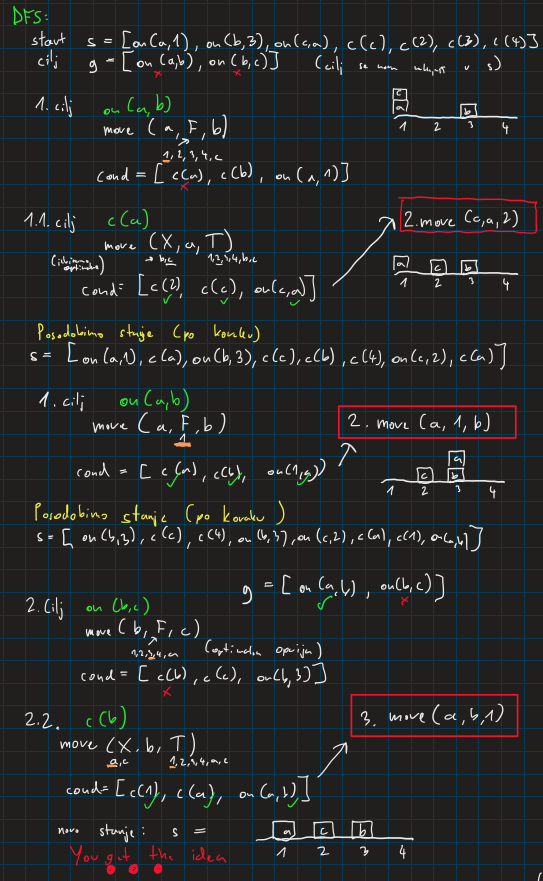
\includegraphics[trim={0cm 0cm 0cm 0cm},clip,width=6.5cm]{strips.png}



\subsection{Planiranje z regresiranjem ciljev (STRIPS)}
Resitev za sussmanovo anomalijo\\
Zacnemo v ciljih, regresiramo do zacetka ($G_i \subset S_0$):

\begin{enumerate}[noitemsep,topsep=0pt,leftmargin=*]
\item $G_{i+1} = G_i \cup \text{cond}(A) - \text{adds}(A)$
\item \blue{POGOJ}: $G_{i} \cap \text{dels}(A) = \emptyset$
\item Preveri da ni protislovja (npr. $G_{i+1} = \left[on(b,c), \dots, c(c) \dots\right]$)
\end{enumerate}
$\rightarrow$ zactno\_stanje = [on(a,1), on(b,a), c(b), on(c,3), c(c)]\\
$\rightarrow$ hocemo da $\text{zacetno\_stanje} \subset G_i$
\begin{enumerate}[noitemsep,topsep=0pt,leftmargin=*,]
    \item $G_0$ = [on(a,b), on(b,c)]
    \begin{itemize}[noitemsep,topsep=0pt,leftmargin=0.5cm]
        \item \green{on(a,b)}: $A_0=move(a, From, b)$
        \item From = 1
        \item POGOJ: $G_0 \cap \text{dels}(A_0) = \emptyset \green{\checkmark}$
        \item $G_1$ = [on(a,b), on(b,c), c(a), c(b), on(a,1)]-[c(1), on(a,b)] $\green{\checkmark}$
    \end{itemize}
    \item $G_1=$[on(b,c),c(a),c(b),on(a,1)]
    \begin{itemize}[noitemsep,topsep=0pt,leftmargin=0.5cm]
        \item \green{c(a)}: $A_1=move(X, a, To)$
        \item X = c, To = 2
        \item POGOJ: $G_1 \cap \text{dels}(A_1) = \emptyset \green{\checkmark}$
        \item $G_2$ = [\underline{on(b,c)},c(a),c(b),on(a,1),\underline{c(c)},c(2),on(c,a)]\\ -[c(a), on(c,2)] \xmark (protislovje)
        \item \green{on(b,c)}: $A_2=move(b, From, c)$
        \item From = 3
        \item POGOJ: $G_2 \cap \text{dels}(A_2) = \emptyset \green{\checkmark}$
        \item $G_2$ = [on(b,c),c(a),c(b),on(a,1),c(c),c(b),on(b,3)] \cmark
    \end{itemize}
    \item $G_2$ = ...     
\end{enumerate}


\subsection{RAZPOREJANJE OPRAVIL (PDDL)}
Razsirimo lahko notacijo (PDDL):\\
\textbf{Akcija1 $\green{\prec}$ Akcija2}: Akcija1 se mora zgoditi pred Akcijo2\\
\textbf{Resources} podajo stevila razpolozljivih resursov\\
\textbf{DURATION} opredejljuje trajanje posamezne akcije\\
\textbf{CONSUME} opredeljuje (trajno) porabo dolocene kolicine resursov\\
\textbf{USE} opredeljuje (zacasno) zasedenost kolicine resursov med izvajanjem akcije\\
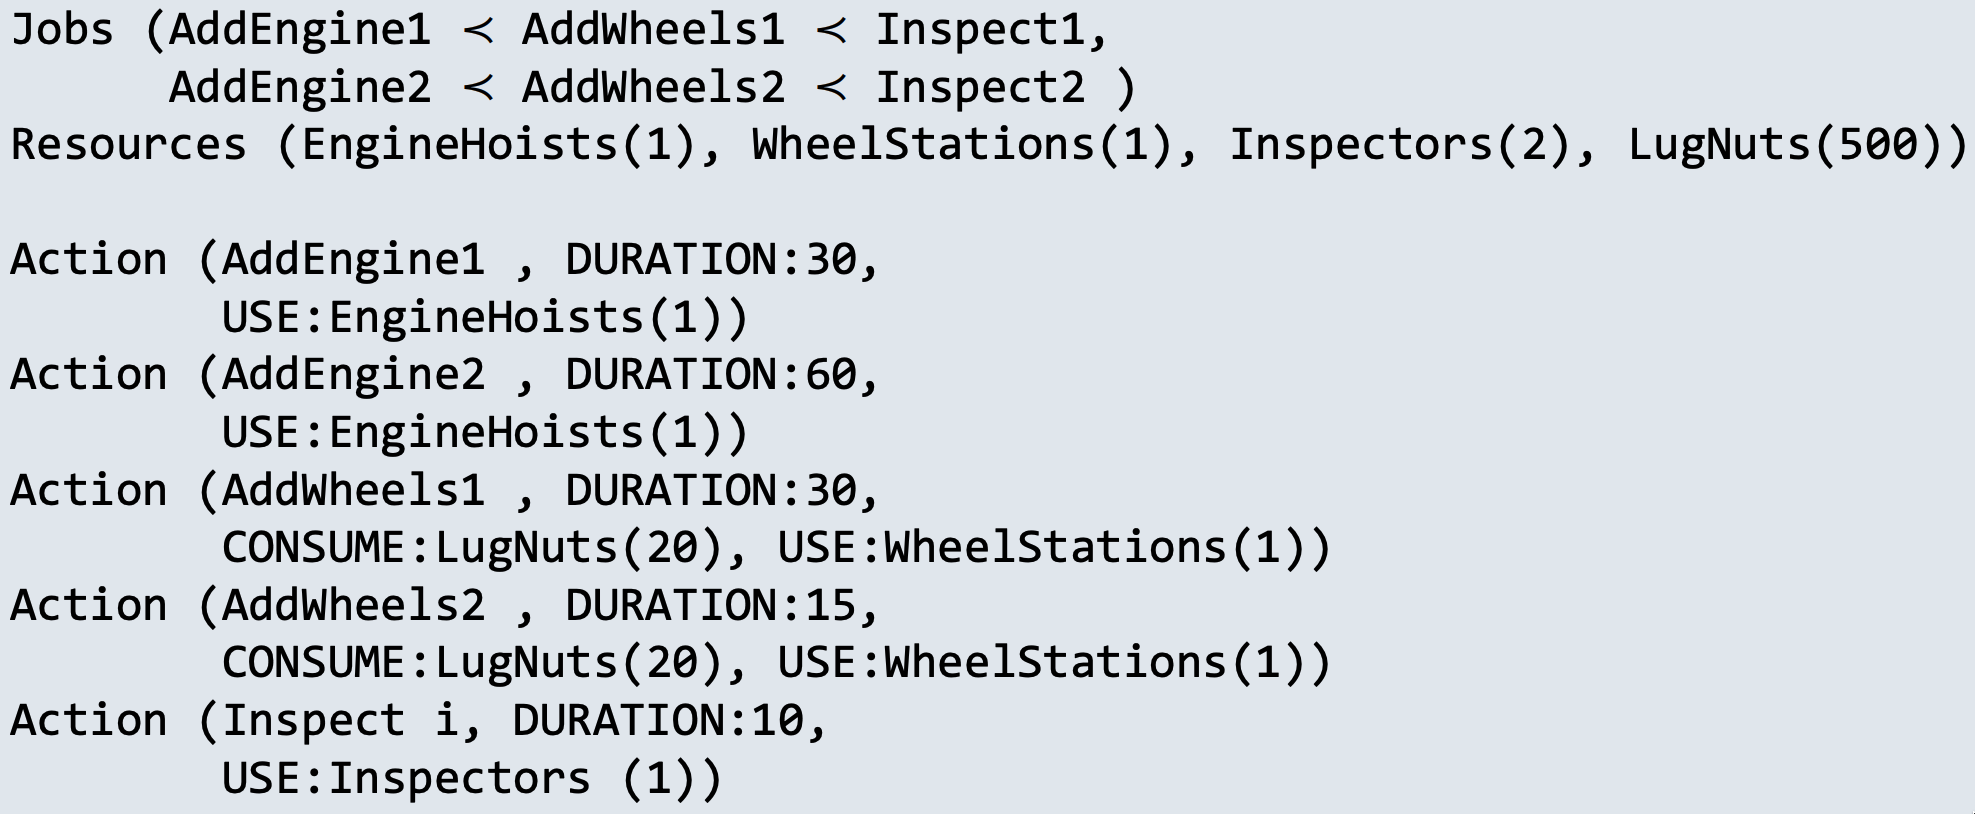
\includegraphics[width=7cm]{./images/pddl.png}
\textbf{Metoda kriticne poti}\\
kriticna pot: pot, ki je \textbf{najdaljsa} in doloca dolzino trajanja celotnega plana
vsaki akciji priredimo par \textbf{[ES, LS]}
\begin{itemize}[leftmargin=*,noitemsep,topsep=0pt]
    \item \textbf{ES}: najbolj zgodnji mozen zacetek (Earliest Start)
    \begin{itemize}[leftmargin=*,noitemsep,topsep=0pt]
        \item $ES(start) = 0$, $\quad ES(B) = \max\limits_{A \prec B} \left[ ES(A) + Duration(A)\right]$
    \end{itemize}
    \item \textbf{LS}: najbolj pozen mozen zacetek (Latest Start)
    \begin{itemize}[leftmargin=*,noitemsep,topsep=0pt]
        \item LS(Finish) = ES(Finish), $LS(A) = \min\limits_{A\prec B}\left[ LS(B) - Duration(A)\right]$
    \end{itemize}
\end{itemize}
\green{rezerva(slack)}=LS-ES (\textbf{casovna rezerva})
\blue{Algoritem} po \textbf{hevristiki \green{minimum slack}} $\rightarrow$ na vsaki iteraciji ima prednost akcija 
ki ima izpolnjene predhodnike in najnizji slack, nato posodobi [ES in LS] za celotni graf in ponovi.

